\setlength{\columnsep}{3pt}
\begin{flushleft}
	\bigskip
	\paragraph{What is SGID?}
	\begin{itemize}
		\item SGID stands for \textbf{S}et \textbf{G}roup \textbf{ID}.
		\item \textbf{SGID can be applied only on directories}.
		\item \textbf{SGID is applicable only on group ownership}.
		\item When SGID permission is set on a directory, all the new (future) files/folders created
		under that directory will have the same group owner as that of the parent
		directory.
		\item Subdirectories created in future will also have SGID bit on them.
		\item SGID is denoted as \textbf{"s"} for group, if group has execute permission:
		\begin{figure}[h!]
			\centering
			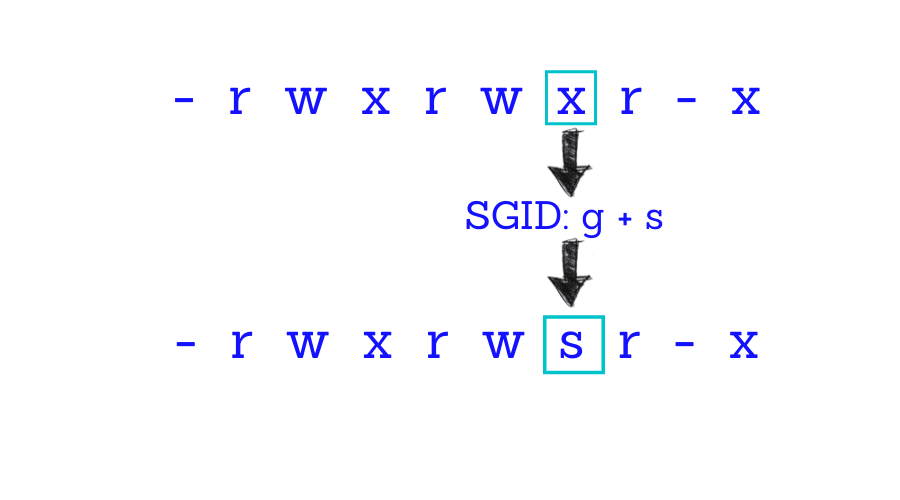
\includegraphics[scale=0.3]{content/chapter6/images/adv_perm3.png}
			\caption{SGID permission}
			\label{fig:combination_permission5}
		\end{figure}
		\item SGID is denoted as \textbf{"S"} for group, if no execute permission is applied for group:
		\begin{figure}[h!]
			\centering
			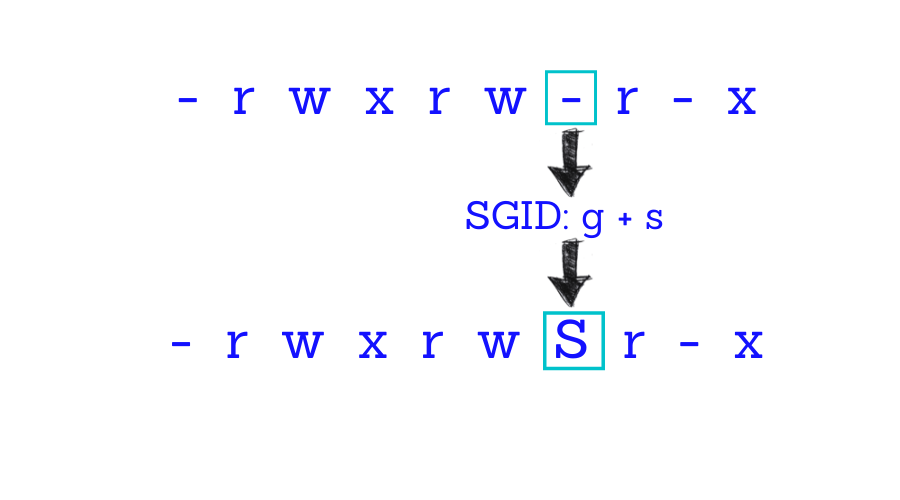
\includegraphics[scale=0.3]{content/chapter6/images/adv_perm4.png}
			\caption{SGID permission}
			\label{fig:combination_permission6}
		\end{figure}
		\item Octal representation of SGID is \textbf{"2"}.
	\end{itemize}
	\newpage	
	\paragraph{How to apply SGID permission?}
	Command:
	\begin{tcolorbox}[breakable,notitle,boxrule=0pt,colback=pink,colframe=pink]
		\color{black}
		\fontdimen2\font=1em
		Syntax: chmod g+s directory\_name
		\fontdimen2\font=4pt
	\end{tcolorbox}
	Eg: Create a folder named \textbf{"/project"} with below conditions:
	\begin{itemize}
		\item Owner: raj
		\item Group: devops
		\item SGUID: yes
	\end{itemize}
	\textbf{Solution}:
	\begin{itemize}
		\item Create the folder:
		\bigskip
		\begin{tcolorbox}[breakable,notitle,boxrule=-0pt,colback=black,colframe=black]
			\color{green}
			\fontdimen2\font=1em
			\# mkdir /project
			\fontdimen2\font=4pt
		\end{tcolorbox}
		\item Assign owner as raj and group as devops:
		\begin{tcolorbox}[breakable,notitle,boxrule=-0pt,colback=black,colframe=black]
			\color{green}
			\fontdimen2\font=1em
			\# chown raj:devops /project
			\fontdimen2\font=4pt
		\end{tcolorbox}
		\item Set SGID on /project folder:
		\begin{tcolorbox}[breakable,notitle,boxrule=-0pt,colback=black,colframe=black]
			\color{green}
			\fontdimen2\font=1em
			\# chmod g+s /project
			\newline
			\color{white}
			or
			\color{green}
			\newline
			\# chmod 2770 /project
			\fontdimen2\font=4pt
		\end{tcolorbox}
		\item To confirm the effect of SGID, switch to root user and create a file named \textbf{"/project/sample.txt"}. Confirm the group ownership is set to \textbf{"devops"}.
		\begin{figure}[h!]
			\centering
			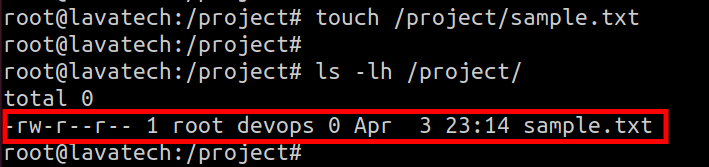
\includegraphics[scale=0.5]{content/chapter6/images/123.png}
			\caption{Sample output}
			\label{fig:combination_permission41}
		\end{figure}
	\end{itemize}
	\newpage
	\paragraph{How to remove SGID permission?}
	\bigskip
	Command:
	\begin{tcolorbox}[breakable,notitle,boxrule=0pt,colback=pink,colframe=pink]
		\color{black}
		\fontdimen2\font=1em
		Syntax: chmod g-s directory\_name
		\fontdimen2\font=4pt
	\end{tcolorbox}
	Eg:
	\begin{tcolorbox}[breakable,notitle,boxrule=-0pt,colback=black,colframe=black]
		\color{green}
		\fontdimen2\font=1em
		\# chmod g-s  /tmp/test
		\newline
		or
		\newline
		\# chmod 0750 /tmp/test
		\fontdimen2\font=4pt
	\end{tcolorbox}
	
	
	
	
	
\end{flushleft}

\newpage

